\section{Desiderata for epidemiological models}
\label{sec:dessiderata}

In what follows, we provide give a non-exhaustive list of requirements we have identified as important when modeling the \acrshort{c19} epidemic. To begin, we present a na\"{i}ve analysis of reproduction numbers and weekly growth factors for the  German data to illustrate where this simple approach breaks down. This will be our starting point to motivate which effects to include in our modeling considerations.

For the reproduction number, we first estimate $\hat R$ by the moment estimator \eqref{eq:hatR} using the raw incidences $I_{t}$ for the whole of Germany and the generation time distribution from \Cref{fig:generation_time}. As these estimates are affected by the weekday effect present in the raw incidences, we repeat the estimation, now based on the seven-day averages $\frac{1}{7}\sum_{\tau = -3}^3I_{t - \tau}$, producing smoother estimates. 
Similarly, we estimate the weekly growth factor once by the raw incidences, $ \hat \rho^{7} = \frac{I_{t}}{I_{t - 7}}$ and the smoothed estimate \Cref{eq:rho7_smooth}.

\begin{figure}
    \resizebox{\textwidth}{!}{%
        % Created by tikzDevice version 0.12.6 on 2025-01-15 07:37:59
% !TEX encoding = UTF-8 Unicode
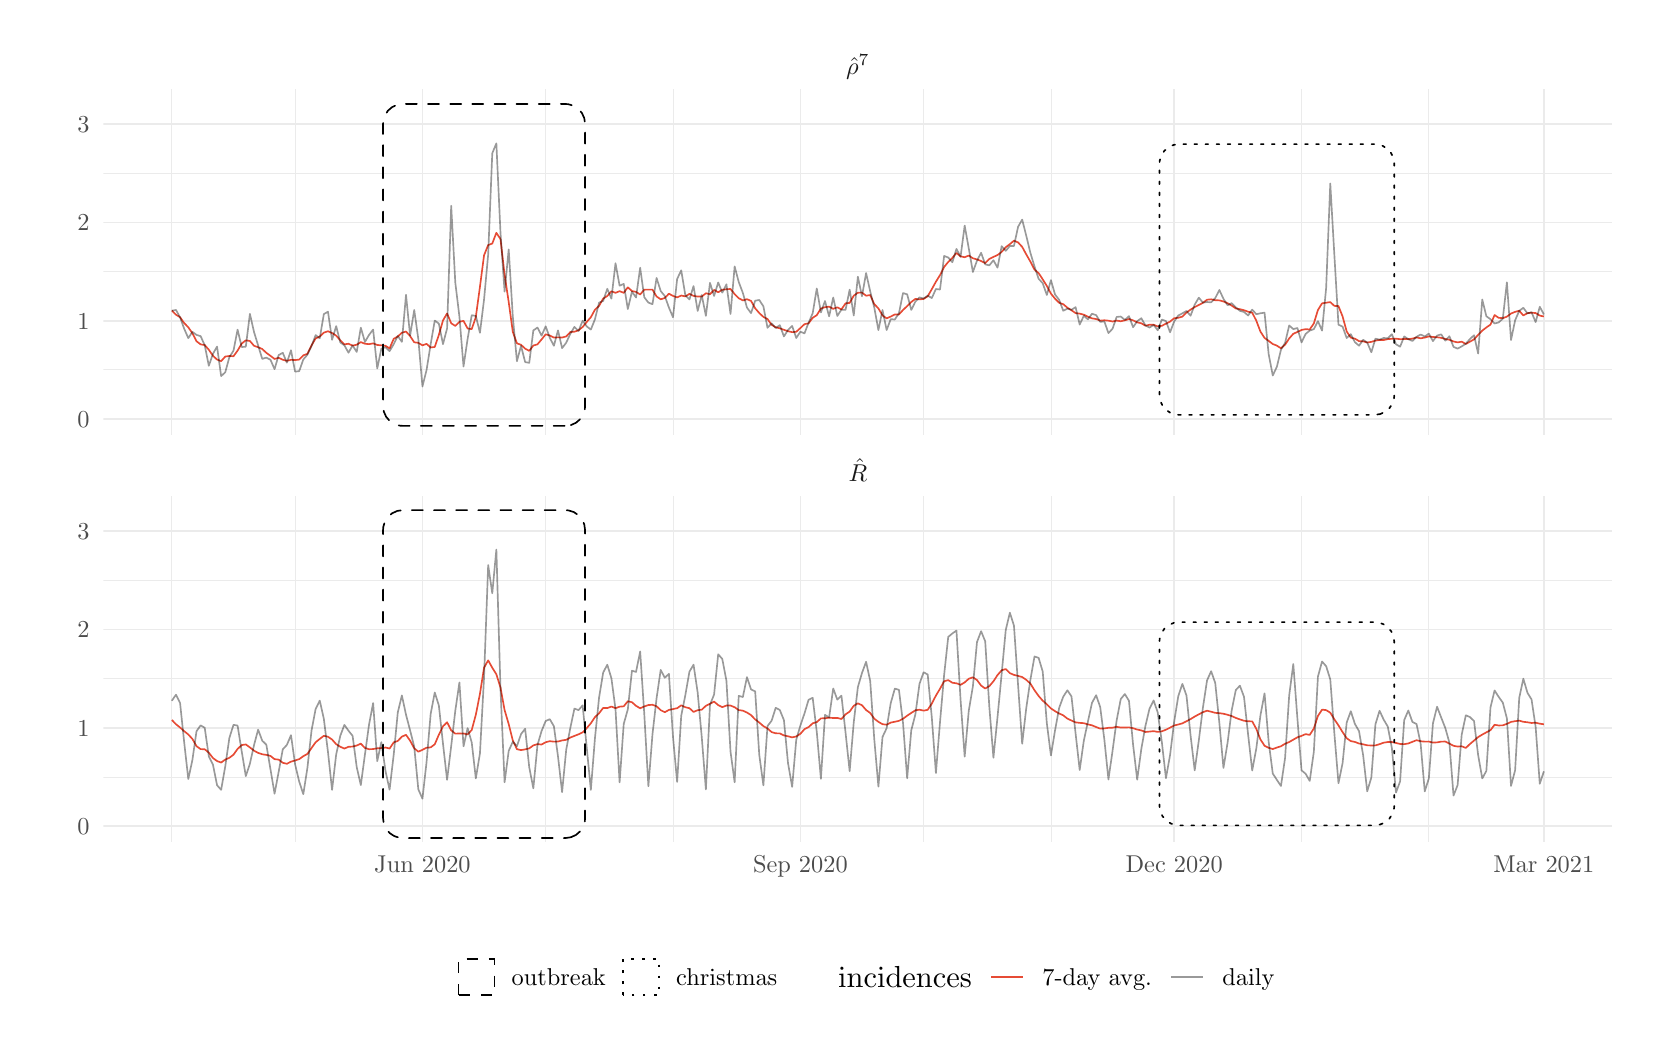
\begin{tikzpicture}[x=1pt,y=1pt]
\definecolor{fillColor}{RGB}{255,255,255}
\path[use as bounding box,fill=fillColor,fill opacity=0.00] (0,0) rectangle (578.16,361.35);
\begin{scope}
\path[clip] ( 27.31,214.24) rectangle (572.66,339.28);
\definecolor{drawColor}{gray}{0.92}

\path[draw=drawColor,line width= 0.3pt,line join=round] ( 27.31,237.69) --
	(572.66,237.69);

\path[draw=drawColor,line width= 0.3pt,line join=round] ( 27.31,273.21) --
	(572.66,273.21);

\path[draw=drawColor,line width= 0.3pt,line join=round] ( 27.31,308.73) --
	(572.66,308.73);

\path[draw=drawColor,line width= 0.3pt,line join=round] ( 52.10,214.24) --
	( 52.10,339.28);

\path[draw=drawColor,line width= 0.3pt,line join=round] ( 96.63,214.24) --
	( 96.63,339.28);

\path[draw=drawColor,line width= 0.3pt,line join=round] (187.18,214.24) --
	(187.18,339.28);

\path[draw=drawColor,line width= 0.3pt,line join=round] (233.19,214.24) --
	(233.19,339.28);

\path[draw=drawColor,line width= 0.3pt,line join=round] (323.74,214.24) --
	(323.74,339.28);

\path[draw=drawColor,line width= 0.3pt,line join=round] (369.75,214.24) --
	(369.75,339.28);

\path[draw=drawColor,line width= 0.3pt,line join=round] (460.30,214.24) --
	(460.30,339.28);

\path[draw=drawColor,line width= 0.3pt,line join=round] (506.31,214.24) --
	(506.31,339.28);

\path[draw=drawColor,line width= 0.6pt,line join=round] ( 27.31,219.93) --
	(572.66,219.93);

\path[draw=drawColor,line width= 0.6pt,line join=round] ( 27.31,255.45) --
	(572.66,255.45);

\path[draw=drawColor,line width= 0.6pt,line join=round] ( 27.31,290.97) --
	(572.66,290.97);

\path[draw=drawColor,line width= 0.6pt,line join=round] ( 27.31,326.49) --
	(572.66,326.49);

\path[draw=drawColor,line width= 0.6pt,line join=round] (142.65,214.24) --
	(142.65,339.28);

\path[draw=drawColor,line width= 0.6pt,line join=round] (279.21,214.24) --
	(279.21,339.28);

\path[draw=drawColor,line width= 0.6pt,line join=round] (414.28,214.24) --
	(414.28,339.28);

\path[draw=drawColor,line width= 0.6pt,line join=round] (547.87,214.24) --
	(547.87,339.28);
\definecolor{drawColor}{RGB}{230,75,53}

\path[draw=drawColor,line width= 0.6pt,line join=round] ( 52.10,259.14) --
	( 53.59,257.63) --
	( 55.07,256.71) --
	( 56.55,254.61) --
	( 58.04,253.09) --
	( 59.52,250.93) --
	( 61.01,248.04) --
	( 62.49,246.91) --
	( 63.98,246.66) --
	( 65.46,244.96) --
	( 66.95,242.80) --
	( 68.43,241.41) --
	( 69.91,240.85) --
	( 71.40,242.51) --
	( 72.88,242.71) --
	( 74.37,242.62) --
	( 75.85,244.65) --
	( 77.34,247.20) --
	( 78.82,248.37) --
	( 80.30,248.13) --
	( 81.79,246.40) --
	( 83.27,245.88) --
	( 84.76,245.23) --
	( 86.24,243.85) --
	( 87.73,242.77) --
	( 89.21,241.63) --
	( 90.69,242.06) --
	( 92.18,241.36) --
	( 93.66,240.96) --
	( 95.15,241.32) --
	( 96.63,241.24) --
	( 98.12,241.40) --
	( 99.60,242.94) --
	(101.08,243.49) --
	(102.57,246.54) --
	(104.05,249.05) --
	(105.54,249.73) --
	(107.02,251.16) --
	(108.51,251.65) --
	(109.99,251.00) --
	(111.48,250.07) --
	(112.96,248.38) --
	(114.44,246.91) --
	(115.93,247.13) --
	(117.41,246.45) --
	(118.90,246.79) --
	(120.38,247.73) --
	(121.87,247.13) --
	(123.35,246.99) --
	(124.83,247.28) --
	(126.32,246.69) --
	(127.80,246.56) --
	(129.29,246.40) --
	(130.77,245.45) --
	(132.26,248.91) --
	(133.74,249.75) --
	(135.22,251.11) --
	(136.71,251.55) --
	(138.19,249.92) --
	(139.68,247.65) --
	(141.16,247.47) --
	(142.65,246.56) --
	(144.13,247.08) --
	(145.62,245.79) --
	(147.10,245.97) --
	(148.58,250.34) --
	(150.07,255.54) --
	(151.55,258.10) --
	(153.04,254.54) --
	(154.52,253.57) --
	(156.01,255.07) --
	(157.49,255.40) --
	(158.97,252.65) --
	(160.46,252.41) --
	(161.94,256.83) --
	(163.43,267.73) --
	(164.91,279.11) --
	(166.40,282.79) --
	(167.88,283.35) --
	(169.36,287.22) --
	(170.85,284.97) --
	(172.33,272.12) --
	(173.82,262.20) --
	(175.30,251.42) --
	(176.79,247.28) --
	(178.27,246.76) --
	(179.76,245.36) --
	(181.24,244.57) --
	(182.72,246.49) --
	(184.21,246.92) --
	(185.69,248.69) --
	(187.18,250.54) --
	(188.66,250.12) --
	(190.15,249.37) --
	(191.63,249.45) --
	(193.11,249.38) --
	(194.60,249.78) --
	(196.08,251.35) --
	(197.57,251.49) --
	(199.05,251.98) --
	(200.54,253.19) --
	(202.02,255.02) --
	(203.50,256.72) --
	(204.99,259.44) --
	(206.47,260.82) --
	(207.96,263.46) --
	(209.44,264.38) --
	(210.93,266.09) --
	(212.41,265.54) --
	(213.89,266.13) --
	(215.38,265.53) --
	(216.86,267.52) --
	(218.35,266.19) --
	(219.83,265.86) --
	(221.32,264.93) --
	(222.80,266.67) --
	(224.29,266.69) --
	(225.77,266.69) --
	(227.25,264.22) --
	(228.74,263.20) --
	(230.22,263.65) --
	(231.71,265.22) --
	(233.19,264.41) --
	(234.68,263.87) --
	(236.16,264.56) --
	(237.64,264.23) --
	(239.13,265.15) --
	(240.61,264.42) --
	(242.10,264.20) --
	(243.58,264.17) --
	(245.07,265.38) --
	(246.55,265.03) --
	(248.03,266.58) --
	(249.52,265.73) --
	(251.00,266.64) --
	(252.49,266.82) --
	(253.97,266.93) --
	(255.46,265.08) --
	(256.94,263.59) --
	(258.43,262.79) --
	(259.91,263.24) --
	(261.39,262.61) --
	(262.88,259.94) --
	(264.36,258.23) --
	(265.85,256.83) --
	(267.33,256.07) --
	(268.82,253.97) --
	(270.30,253.08) --
	(271.78,252.72) --
	(273.27,252.16) --
	(274.75,251.67) --
	(276.24,251.32) --
	(277.72,251.45) --
	(279.21,252.80) --
	(280.69,254.21) --
	(282.17,254.51) --
	(283.66,256.50) --
	(285.14,257.46) --
	(286.63,259.86) --
	(288.11,260.34) --
	(289.60,260.54) --
	(291.08,259.75) --
	(292.56,260.30) --
	(294.05,259.53) --
	(295.53,261.73) --
	(297.02,261.89) --
	(298.50,264.50) --
	(299.99,265.58) --
	(301.47,265.61) --
	(302.96,264.49) --
	(304.44,264.73) --
	(305.92,261.45) --
	(307.41,259.91) --
	(308.89,257.36) --
	(310.38,256.31) --
	(311.86,256.95) --
	(313.35,257.71) --
	(314.83,257.73) --
	(316.31,259.34) --
	(317.80,260.74) --
	(319.28,262.21) --
	(320.77,263.34) --
	(322.25,263.16) --
	(323.74,263.31) --
	(325.22,264.28) --
	(326.70,266.85) --
	(328.19,269.54) --
	(329.67,271.94) --
	(331.16,274.89) --
	(332.64,276.69) --
	(334.13,278.18) --
	(335.61,279.94) --
	(337.10,278.70) --
	(338.58,278.40) --
	(340.06,279.00) --
	(341.55,278.02) --
	(343.03,277.60) --
	(344.52,277.03) --
	(346.00,276.28) --
	(347.49,277.77) --
	(348.97,278.51) --
	(350.45,279.18) --
	(351.94,280.31) --
	(353.42,282.01) --
	(354.91,283.13) --
	(356.39,284.38) --
	(357.88,283.74) --
	(359.36,282.14) --
	(360.84,279.41) --
	(362.33,276.80) --
	(363.81,273.92) --
	(365.30,272.65) --
	(366.78,270.41) --
	(368.27,268.02) --
	(369.75,265.25) --
	(371.23,263.42) --
	(372.72,261.93) --
	(374.20,261.43) --
	(375.69,260.15) --
	(377.17,259.25) --
	(378.66,258.20) --
	(380.14,258.02) --
	(381.63,257.63) --
	(383.11,256.91) --
	(384.59,256.31) --
	(386.08,256.06) --
	(387.56,255.48) --
	(389.05,255.62) --
	(390.53,255.47) --
	(392.02,255.17) --
	(393.50,255.51) --
	(394.98,255.26) --
	(396.47,255.60) --
	(397.95,256.07) --
	(399.44,255.58) --
	(400.92,254.86) --
	(402.41,254.52) --
	(403.89,253.66) --
	(405.37,253.99) --
	(406.86,253.99) --
	(408.34,253.40) --
	(409.83,253.62) --
	(411.31,254.39) --
	(412.80,255.15) --
	(414.28,256.35) --
	(415.77,256.52) --
	(417.25,256.94) --
	(418.73,258.39) --
	(420.22,259.48) --
	(421.70,260.38) --
	(423.19,261.13) --
	(424.67,261.92) --
	(426.16,263.04) --
	(427.64,263.19) --
	(429.12,262.86) --
	(430.61,262.81) --
	(432.09,262.41) --
	(433.58,261.78) --
	(435.06,260.93) --
	(436.55,259.88) --
	(438.03,259.62) --
	(439.51,259.25) --
	(441.00,258.71) --
	(442.48,258.38) --
	(443.97,255.45) --
	(445.45,251.53) --
	(446.94,249.24) --
	(448.42,248.17) --
	(449.91,247.04) --
	(451.39,246.45) --
	(452.87,245.50) --
	(454.36,246.81) --
	(455.84,249.04) --
	(457.33,250.73) --
	(458.81,251.39) --
	(460.30,252.11) --
	(461.78,252.41) --
	(463.26,252.28) --
	(464.75,254.48) --
	(466.23,259.33) --
	(467.72,261.73) --
	(469.20,261.96) --
	(470.69,262.18) --
	(472.17,260.81) --
	(473.65,260.74) --
	(475.14,256.99) --
	(476.62,251.59) --
	(478.11,249.35) --
	(479.59,248.97) --
	(481.08,248.08) --
	(482.56,248.00) --
	(484.04,247.58) --
	(485.53,247.81) --
	(487.01,248.27) --
	(488.50,248.49) --
	(489.98,248.47) --
	(491.47,248.80) --
	(492.95,248.92) --
	(494.44,248.97) --
	(495.92,248.78) --
	(497.40,248.85) --
	(498.89,248.81) --
	(500.37,248.99) --
	(501.86,249.41) --
	(503.34,249.10) --
	(504.83,249.35) --
	(506.31,249.79) --
	(507.79,249.58) --
	(509.28,249.48) --
	(510.76,249.28) --
	(512.25,248.85) --
	(513.73,248.57) --
	(515.22,247.97) --
	(516.70,247.62) --
	(518.18,247.88) --
	(519.67,247.04) --
	(521.15,247.88) --
	(522.64,248.72) --
	(524.12,250.36) --
	(525.61,251.87) --
	(527.09,253.02) --
	(528.58,254.06) --
	(530.06,257.51) --
	(531.54,256.50) --
	(533.03,256.38) --
	(534.51,256.93) --
	(536.00,258.05) --
	(537.48,258.66) --
	(538.97,259.05) --
	(540.45,257.36) --
	(541.93,258.18) --
	(543.42,258.36) --
	(544.90,258.22) --
	(546.39,257.31) --
	(547.87,256.99);
\definecolor{drawColor}{RGB}{0,0,0}

\path[draw=drawColor,draw opacity=0.40,line width= 0.6pt,line join=round] ( 52.10,259.07) --
	( 53.59,259.34) --
	( 55.07,256.67) --
	( 56.55,252.57) --
	( 58.04,249.16) --
	( 59.52,251.43) --
	( 61.01,250.33) --
	( 62.49,249.88) --
	( 63.98,246.59) --
	( 65.46,239.17) --
	( 66.95,243.49) --
	( 68.43,246.12) --
	( 69.91,235.44) --
	( 71.40,236.83) --
	( 72.88,242.29) --
	( 74.37,244.63) --
	( 75.85,252.25) --
	( 77.34,245.94) --
	( 78.82,246.08) --
	( 80.30,257.94) --
	( 81.79,251.38) --
	( 83.27,246.53) --
	( 84.76,241.67) --
	( 86.24,242.12) --
	( 87.73,241.36) --
	( 89.21,237.95) --
	( 90.69,243.04) --
	( 92.18,243.86) --
	( 93.66,240.30) --
	( 95.15,244.79) --
	( 96.63,237.05) --
	( 98.12,237.24) --
	( 99.60,241.45) --
	(101.08,243.17) --
	(102.57,246.31) --
	(104.05,250.25) --
	(105.54,249.12) --
	(107.02,257.85) --
	(108.51,258.71) --
	(109.99,248.56) --
	(111.48,253.50) --
	(112.96,247.62) --
	(114.44,246.56) --
	(115.93,243.90) --
	(117.41,246.53) --
	(118.90,244.17) --
	(120.38,252.95) --
	(121.87,247.77) --
	(123.35,250.33) --
	(124.83,252.26) --
	(126.32,238.21) --
	(127.80,245.38) --
	(129.29,245.84) --
	(130.77,244.47) --
	(132.26,246.96) --
	(133.74,249.95) --
	(135.22,247.81) --
	(136.71,264.80) --
	(138.19,250.05) --
	(139.68,259.35) --
	(141.16,248.80) --
	(142.65,231.68) --
	(144.13,237.60) --
	(145.62,246.96) --
	(147.10,255.52) --
	(148.58,254.41) --
	(150.07,247.00) --
	(151.55,252.66) --
	(153.04,296.98) --
	(154.52,269.22) --
	(156.01,256.95) --
	(157.49,238.93) --
	(158.97,248.89) --
	(160.46,257.44) --
	(161.94,257.18) --
	(163.43,251.11) --
	(164.91,263.12) --
	(166.40,279.38) --
	(167.88,315.95) --
	(169.36,319.55) --
	(170.85,287.19) --
	(172.33,265.98) --
	(173.82,281.23) --
	(175.30,256.96) --
	(176.79,240.82) --
	(178.27,246.39) --
	(179.76,240.49) --
	(181.24,240.24) --
	(182.72,251.94) --
	(184.21,252.99) --
	(185.69,250.06) --
	(187.18,253.43) --
	(188.66,249.28) --
	(190.15,246.40) --
	(191.63,251.96) --
	(193.11,245.55) --
	(194.60,247.51) --
	(196.08,250.72) --
	(197.57,253.23) --
	(199.05,251.75) --
	(200.54,255.45) --
	(202.02,253.40) --
	(203.50,252.26) --
	(204.99,256.00) --
	(206.47,261.98) --
	(207.96,262.62) --
	(209.44,266.98) --
	(210.93,263.44) --
	(212.41,276.22) --
	(213.89,268.10) --
	(215.38,268.77) --
	(216.86,259.68) --
	(218.35,265.94) --
	(219.83,263.84) --
	(221.32,274.60) --
	(222.80,263.95) --
	(224.29,262.00) --
	(225.77,261.43) --
	(227.25,270.91) --
	(228.74,266.18) --
	(230.22,264.39) --
	(231.71,260.21) --
	(233.19,256.69) --
	(234.68,270.53) --
	(236.16,273.65) --
	(237.64,264.67) --
	(239.13,263.14) --
	(240.61,267.97) --
	(242.10,258.99) --
	(243.58,264.72) --
	(245.07,257.21) --
	(246.55,269.13) --
	(248.03,264.41) --
	(249.52,269.28) --
	(251.00,265.59) --
	(252.49,268.61) --
	(253.97,257.90) --
	(255.46,275.06) --
	(256.94,269.45) --
	(258.43,265.50) --
	(259.91,260.21) --
	(261.39,258.19) --
	(262.88,262.70) --
	(264.36,262.94) --
	(265.85,260.65) --
	(267.33,252.89) --
	(268.82,254.52) --
	(270.30,252.79) --
	(271.78,253.85) --
	(273.27,249.77) --
	(274.75,252.13) --
	(276.24,253.56) --
	(277.72,249.21) --
	(279.21,251.49) --
	(280.69,250.87) --
	(282.17,254.71) --
	(283.66,258.15) --
	(285.14,267.09) --
	(286.63,258.44) --
	(288.11,262.57) --
	(289.60,257.03) --
	(291.08,263.83) --
	(292.56,257.18) --
	(294.05,259.46) --
	(295.53,259.37) --
	(297.02,266.68) --
	(298.50,257.36) --
	(299.99,271.34) --
	(301.47,264.28) --
	(302.96,272.68) --
	(304.44,266.10) --
	(305.92,260.19) --
	(307.41,252.05) --
	(308.89,259.31) --
	(310.38,252.09) --
	(311.86,256.02) --
	(313.35,255.89) --
	(314.83,258.17) --
	(316.31,265.45) --
	(317.80,264.99) --
	(319.28,259.36) --
	(320.77,262.36) --
	(322.25,263.87) --
	(323.74,263.48) --
	(325.22,264.52) --
	(326.70,263.65) --
	(328.19,266.91) --
	(329.67,266.73) --
	(331.16,278.86) --
	(332.64,278.29) --
	(334.13,276.60) --
	(335.61,281.40) --
	(337.10,278.58) --
	(338.58,289.83) --
	(340.06,281.59) --
	(341.55,273.07) --
	(343.03,277.14) --
	(344.52,280.00) --
	(346.00,275.83) --
	(347.49,275.46) --
	(348.97,277.31) --
	(350.45,274.62) --
	(351.94,282.38) --
	(353.42,280.70) --
	(354.91,282.44) --
	(356.39,282.48) --
	(357.88,289.40) --
	(359.36,291.98) --
	(360.84,286.13) --
	(362.33,279.97) --
	(363.81,275.07) --
	(365.30,270.61) --
	(366.78,269.00) --
	(368.27,264.75) --
	(369.75,270.13) --
	(371.23,264.93) --
	(372.72,263.01) --
	(374.20,259.06) --
	(375.69,259.82) --
	(377.17,259.40) --
	(378.66,260.36) --
	(380.14,254.07) --
	(381.63,257.21) --
	(383.11,255.96) --
	(384.59,257.97) --
	(386.08,257.49) --
	(387.56,255.05) --
	(389.05,255.19) --
	(390.53,250.97) --
	(392.02,252.57) --
	(393.50,256.83) --
	(394.98,256.96) --
	(396.47,255.74) --
	(397.95,257.11) --
	(399.44,253.11) --
	(400.92,255.29) --
	(402.41,256.35) --
	(403.89,253.76) --
	(405.37,252.98) --
	(406.86,253.93) --
	(408.34,252.01) --
	(409.83,255.88) --
	(411.31,255.33) --
	(412.80,251.27) --
	(414.28,255.19) --
	(415.77,257.34) --
	(417.25,258.12) --
	(418.73,258.98) --
	(420.22,257.27) --
	(421.70,261.27) --
	(423.19,263.77) --
	(424.67,261.99) --
	(426.16,262.21) --
	(427.64,262.10) --
	(429.12,263.61) --
	(430.61,266.57) --
	(432.09,263.37) --
	(433.58,261.07) --
	(435.06,261.81) --
	(436.55,260.28) --
	(438.03,259.04) --
	(439.51,258.62) --
	(441.00,257.35) --
	(442.48,259.46) --
	(443.97,257.81) --
	(445.45,258.14) --
	(446.94,258.36) --
	(448.42,243.40) --
	(449.91,235.66) --
	(451.39,238.81) --
	(452.87,244.97) --
	(454.36,247.43) --
	(455.84,253.74) --
	(457.33,252.43) --
	(458.81,252.82) --
	(460.30,247.61) --
	(461.78,250.68) --
	(463.26,251.88) --
	(464.75,252.41) --
	(466.23,255.28) --
	(467.72,251.88) --
	(469.20,267.31) --
	(470.69,305.03) --
	(472.17,279.13) --
	(473.65,254.02) --
	(475.14,253.32) --
	(476.62,249.19) --
	(478.11,250.59) --
	(479.59,247.70) --
	(481.08,246.43) --
	(482.56,248.55) --
	(484.04,247.58) --
	(485.53,244.06) --
	(487.01,248.97) --
	(488.50,248.61) --
	(489.98,249.22) --
	(491.47,249.09) --
	(492.95,250.55) --
	(494.44,246.94) --
	(495.92,246.07) --
	(497.40,249.78) --
	(498.89,248.78) --
	(500.37,248.14) --
	(501.86,249.62) --
	(503.34,250.47) --
	(504.83,249.76) --
	(506.31,250.79) --
	(507.79,248.09) --
	(509.28,250.08) --
	(510.76,250.53) --
	(512.25,248.26) --
	(513.73,249.84) --
	(515.22,246.01) --
	(516.70,245.37) --
	(518.18,246.18) --
	(519.67,247.13) --
	(521.15,248.84) --
	(522.64,250.19) --
	(524.12,243.61) --
	(525.61,263.13) --
	(527.09,257.06) --
	(528.58,256.00) --
	(530.06,254.45) --
	(531.54,254.84) --
	(533.03,256.19) --
	(534.51,269.34) --
	(536.00,248.47) --
	(537.48,255.59) --
	(538.97,259.04) --
	(540.45,260.12) --
	(541.93,258.11) --
	(543.42,258.52) --
	(544.90,254.95) --
	(546.39,260.50) --
	(547.87,257.73);
\definecolor{drawColor}{RGB}{0,0,0}

\path[draw=drawColor,line width= 0.6pt,dash pattern=on 4pt off 4pt ,line join=round,line cap=round] (196.28,217.74) --
	(198.11,218.57) --
	(199.63,219.87) --
	(200.73,221.55) --
	(201.32,223.47) --
	(201.40,224.57) --
	(201.40,326.66) --
	(201.12,328.65) --
	(200.29,330.48) --
	(198.99,332.00) --
	(197.31,333.10) --
	(195.39,333.69) --
	(194.29,333.77) --
	(135.53,333.77) --
	(133.55,333.49) --
	(131.72,332.66) --
	(130.19,331.36) --
	(129.09,329.68) --
	(128.51,327.76) --
	(128.42,326.66) --
	(128.42,224.57) --
	(128.70,222.58) --
	(129.53,220.75) --
	(130.83,219.23) --
	(132.51,218.13) --
	(134.43,217.54) --
	(135.53,217.46) --
	(194.29,217.46) --
	cycle;

\path[draw=drawColor,line width= 0.6pt,dash pattern=on 1pt off 3pt ,line join=round,line cap=round] (488.69,221.71) --
	(490.52,222.54) --
	(492.05,223.84) --
	(493.15,225.52) --
	(493.73,227.44) --
	(493.82,228.54) --
	(493.82,312.15) --
	(493.54,314.13) --
	(492.71,315.96) --
	(491.40,317.49) --
	(489.73,318.59) --
	(487.81,319.17) --
	(486.71,319.26) --
	(416.07,319.26) --
	(414.09,318.98) --
	(412.26,318.15) --
	(410.73,316.84) --
	(409.63,315.17) --
	(409.05,313.25) --
	(408.96,312.15) --
	(408.96,228.54) --
	(409.24,226.56) --
	(410.07,224.73) --
	(411.38,223.20) --
	(413.05,222.10) --
	(414.97,221.51) --
	(416.07,221.43) --
	(486.71,221.43) --
	cycle;
\end{scope}
\begin{scope}
\path[clip] ( 27.31, 67.14) rectangle (572.66,192.17);
\definecolor{drawColor}{gray}{0.92}

\path[draw=drawColor,line width= 0.3pt,line join=round] ( 27.31, 90.58) --
	(572.66, 90.58);

\path[draw=drawColor,line width= 0.3pt,line join=round] ( 27.31,126.10) --
	(572.66,126.10);

\path[draw=drawColor,line width= 0.3pt,line join=round] ( 27.31,161.63) --
	(572.66,161.63);

\path[draw=drawColor,line width= 0.3pt,line join=round] ( 52.10, 67.14) --
	( 52.10,192.17);

\path[draw=drawColor,line width= 0.3pt,line join=round] ( 96.63, 67.14) --
	( 96.63,192.17);

\path[draw=drawColor,line width= 0.3pt,line join=round] (187.18, 67.14) --
	(187.18,192.17);

\path[draw=drawColor,line width= 0.3pt,line join=round] (233.19, 67.14) --
	(233.19,192.17);

\path[draw=drawColor,line width= 0.3pt,line join=round] (323.74, 67.14) --
	(323.74,192.17);

\path[draw=drawColor,line width= 0.3pt,line join=round] (369.75, 67.14) --
	(369.75,192.17);

\path[draw=drawColor,line width= 0.3pt,line join=round] (460.30, 67.14) --
	(460.30,192.17);

\path[draw=drawColor,line width= 0.3pt,line join=round] (506.31, 67.14) --
	(506.31,192.17);

\path[draw=drawColor,line width= 0.6pt,line join=round] ( 27.31, 72.82) --
	(572.66, 72.82);

\path[draw=drawColor,line width= 0.6pt,line join=round] ( 27.31,108.34) --
	(572.66,108.34);

\path[draw=drawColor,line width= 0.6pt,line join=round] ( 27.31,143.86) --
	(572.66,143.86);

\path[draw=drawColor,line width= 0.6pt,line join=round] ( 27.31,179.39) --
	(572.66,179.39);

\path[draw=drawColor,line width= 0.6pt,line join=round] (142.65, 67.14) --
	(142.65,192.17);

\path[draw=drawColor,line width= 0.6pt,line join=round] (279.21, 67.14) --
	(279.21,192.17);

\path[draw=drawColor,line width= 0.6pt,line join=round] (414.28, 67.14) --
	(414.28,192.17);

\path[draw=drawColor,line width= 0.6pt,line join=round] (547.87, 67.14) --
	(547.87,192.17);
\definecolor{drawColor}{RGB}{230,75,53}

\path[draw=drawColor,line width= 0.6pt,line join=round] ( 52.10,111.18) --
	( 53.59,109.65) --
	( 55.07,108.46) --
	( 56.55,107.14) --
	( 58.04,105.95) --
	( 59.52,104.33) --
	( 61.01,101.72) --
	( 62.49,100.65) --
	( 63.98,100.61) --
	( 65.46, 99.35) --
	( 66.95, 97.44) --
	( 68.43, 96.34) --
	( 69.91, 95.81) --
	( 71.40, 96.88) --
	( 72.88, 97.52) --
	( 74.37, 98.64) --
	( 75.85,100.72) --
	( 77.34,102.11) --
	( 78.82,102.35) --
	( 80.30,101.27) --
	( 81.79,100.09) --
	( 83.27, 99.29) --
	( 84.76, 98.79) --
	( 86.24, 98.56) --
	( 87.73, 98.20) --
	( 89.21, 97.03) --
	( 90.69, 96.86) --
	( 92.18, 95.71) --
	( 93.66, 95.36) --
	( 95.15, 96.12) --
	( 96.63, 96.56) --
	( 98.12, 97.04) --
	( 99.60, 98.10) --
	(101.08, 98.92) --
	(102.57,101.05) --
	(104.05,103.13) --
	(105.54,104.34) --
	(107.02,105.46) --
	(108.51,105.13) --
	(109.99,104.12) --
	(111.48,102.45) --
	(112.96,101.51) --
	(114.44,100.86) --
	(115.93,101.49) --
	(117.41,101.58) --
	(118.90,101.95) --
	(120.38,102.63) --
	(121.87,101.07) --
	(123.35,100.62) --
	(124.83,100.68) --
	(126.32,100.94) --
	(127.80,101.02) --
	(129.29,101.23) --
	(130.77,100.87) --
	(132.26,103.09) --
	(133.74,103.61) --
	(135.22,105.16) --
	(136.71,105.82) --
	(138.19,103.70) --
	(139.68,100.95) --
	(141.16, 99.73) --
	(142.65,100.39) --
	(144.13,101.18) --
	(145.62,101.29) --
	(147.10,102.40) --
	(148.58,105.86) --
	(150.07,108.89) --
	(151.55,110.35) --
	(153.04,107.42) --
	(154.52,106.25) --
	(156.01,106.29) --
	(157.49,106.32) --
	(158.97,105.97) --
	(160.46,107.57) --
	(161.94,113.08) --
	(163.43,120.63) --
	(164.91,130.10) --
	(166.40,132.72) --
	(167.88,130.06) --
	(169.36,127.69) --
	(170.85,122.90) --
	(172.33,114.79) --
	(173.82,109.69) --
	(175.30,103.80) --
	(176.79,100.64) --
	(178.27,100.29) --
	(179.76,100.56) --
	(181.24,100.92) --
	(182.72,102.00) --
	(184.21,102.46) --
	(185.69,102.31) --
	(187.18,103.15) --
	(188.66,103.53) --
	(190.15,103.35) --
	(191.63,103.40) --
	(193.11,103.80) --
	(194.60,104.01) --
	(196.08,104.84) --
	(197.57,105.43) --
	(199.05,106.00) --
	(200.54,106.71) --
	(202.02,108.25) --
	(203.50,109.99) --
	(204.99,112.22) --
	(206.47,113.60) --
	(207.96,115.55) --
	(209.44,115.48) --
	(210.93,116.04) --
	(212.41,115.44) --
	(213.89,115.99) --
	(215.38,116.12) --
	(216.86,117.95) --
	(218.35,117.60) --
	(219.83,116.29) --
	(221.32,115.41) --
	(222.80,116.06) --
	(224.29,116.58) --
	(225.77,116.68) --
	(227.25,116.13) --
	(228.74,114.73) --
	(230.22,113.99) --
	(231.71,114.82) --
	(233.19,115.13) --
	(234.68,115.44) --
	(236.16,116.48) --
	(237.64,115.80) --
	(239.13,115.44) --
	(240.61,114.10) --
	(242.10,114.71) --
	(243.58,114.92) --
	(245.07,116.30) --
	(246.55,117.04) --
	(248.03,117.82) --
	(249.52,116.56) --
	(251.00,115.82) --
	(252.49,116.40) --
	(253.97,116.40) --
	(255.46,115.79) --
	(256.94,114.76) --
	(258.43,114.55) --
	(259.91,113.88) --
	(261.39,112.94) --
	(262.88,111.38) --
	(264.36,110.26) --
	(265.85,108.96) --
	(267.33,108.12) --
	(268.82,106.81) --
	(270.30,106.37) --
	(271.78,106.33) --
	(273.27,105.60) --
	(274.75,105.30) --
	(276.24,104.89) --
	(277.72,105.23) --
	(279.21,106.18) --
	(280.69,107.86) --
	(282.17,108.60) --
	(283.66,109.98) --
	(285.14,110.42) --
	(286.63,111.76) --
	(288.11,111.81) --
	(289.60,112.02) --
	(291.08,111.90) --
	(292.56,111.93) --
	(294.05,111.53) --
	(295.53,113.23) --
	(297.02,114.21) --
	(298.50,116.32) --
	(299.99,117.20) --
	(301.47,116.51) --
	(302.96,114.78) --
	(304.44,113.72) --
	(305.92,111.65) --
	(307.41,110.51) --
	(308.89,109.66) --
	(310.38,109.48) --
	(311.86,110.24) --
	(313.35,110.54) --
	(314.83,110.87) --
	(316.31,111.62) --
	(317.80,112.73) --
	(319.28,113.72) --
	(320.77,114.68) --
	(322.25,114.90) --
	(323.74,114.56) --
	(325.22,114.85) --
	(326.70,117.11) --
	(328.19,120.00) --
	(329.67,122.46) --
	(331.16,125.19) --
	(332.64,125.59) --
	(334.13,124.64) --
	(335.61,124.44) --
	(337.10,123.89) --
	(338.58,124.76) --
	(340.06,126.09) --
	(341.55,126.60) --
	(343.03,125.62) --
	(344.52,123.61) --
	(346.00,122.55) --
	(347.49,123.40) --
	(348.97,125.17) --
	(350.45,127.41) --
	(351.94,129.14) --
	(353.42,129.58) --
	(354.91,128.11) --
	(356.39,127.47) --
	(357.88,127.11) --
	(359.36,126.70) --
	(360.84,125.68) --
	(362.33,124.33) --
	(363.81,121.93) --
	(365.30,119.86) --
	(366.78,118.16) --
	(368.27,116.86) --
	(369.75,115.37) --
	(371.23,114.36) --
	(372.72,113.53) --
	(374.20,112.87) --
	(375.69,111.67) --
	(377.17,110.99) --
	(378.66,110.32) --
	(380.14,110.14) --
	(381.63,110.03) --
	(383.11,109.59) --
	(384.59,109.25) --
	(386.08,108.63) --
	(387.56,108.06) --
	(389.05,108.14) --
	(390.53,108.35) --
	(392.02,108.40) --
	(393.50,108.71) --
	(394.98,108.45) --
	(396.47,108.44) --
	(397.95,108.52) --
	(399.44,108.22) --
	(400.92,107.73) --
	(402.41,107.42) --
	(403.89,106.85) --
	(405.37,106.99) --
	(406.86,107.15) --
	(408.34,106.88) --
	(409.83,107.09) --
	(411.31,107.67) --
	(412.80,108.41) --
	(414.28,109.20) --
	(415.77,109.55) --
	(417.25,109.96) --
	(418.73,110.73) --
	(420.22,111.51) --
	(421.70,112.42) --
	(423.19,113.23) --
	(424.67,114.00) --
	(426.16,114.53) --
	(427.64,114.17) --
	(429.12,113.76) --
	(430.61,113.65) --
	(432.09,113.43) --
	(433.58,113.06) --
	(435.06,112.61) --
	(436.55,111.93) --
	(438.03,111.39) --
	(439.51,110.91) --
	(441.00,110.70) --
	(442.48,110.69) --
	(443.97,107.95) --
	(445.45,104.16) --
	(446.94,101.88) --
	(448.42,101.14) --
	(449.91,100.68) --
	(451.39,101.22) --
	(452.87,101.69) --
	(454.36,102.60) --
	(455.84,103.22) --
	(457.33,104.07) --
	(458.81,104.92) --
	(460.30,105.44) --
	(461.78,106.09) --
	(463.26,105.78) --
	(464.75,108.10) --
	(466.23,112.65) --
	(467.72,114.92) --
	(469.20,114.75) --
	(470.69,113.82) --
	(472.17,111.41) --
	(473.65,109.24) --
	(475.14,106.79) --
	(476.62,104.58) --
	(478.11,103.56) --
	(479.59,103.25) --
	(481.08,102.68) --
	(482.56,102.39) --
	(484.04,102.03) --
	(485.53,101.97) --
	(487.01,102.00) --
	(488.50,102.44) --
	(489.98,102.98) --
	(491.47,103.21) --
	(492.95,103.21) --
	(494.44,102.87) --
	(495.92,102.52) --
	(497.40,102.45) --
	(498.89,102.70) --
	(500.37,103.29) --
	(501.86,103.88) --
	(503.34,103.50) --
	(504.83,103.36) --
	(506.31,103.38) --
	(507.79,103.03) --
	(509.28,103.09) --
	(510.76,103.36) --
	(512.25,103.39) --
	(513.73,102.64) --
	(515.22,101.86) --
	(516.70,101.58) --
	(518.18,101.68) --
	(519.67,101.08) --
	(521.15,102.49) --
	(522.64,103.75) --
	(524.12,105.00) --
	(525.61,105.91) --
	(527.09,106.71) --
	(528.58,107.51) --
	(530.06,109.45) --
	(531.54,109.20) --
	(533.03,109.25) --
	(534.51,109.79) --
	(536.00,110.48) --
	(537.48,110.75) --
	(538.97,110.96) --
	(540.45,110.52) --
	(541.93,110.36) --
	(543.42,110.10) --
	(544.90,110.20) --
	(546.39,109.84) --
	(547.87,109.63);
\definecolor{drawColor}{RGB}{0,0,0}

\path[draw=drawColor,draw opacity=0.40,line width= 0.6pt,line join=round] ( 52.10,118.13) --
	( 53.59,120.32) --
	( 55.07,117.31) --
	( 56.55,103.16) --
	( 58.04, 89.84) --
	( 59.52, 96.71) --
	( 61.01,107.12) --
	( 62.49,109.24) --
	( 63.98,108.36) --
	( 65.46, 98.01) --
	( 66.95, 95.05) --
	( 68.43, 87.61) --
	( 69.91, 85.94) --
	( 71.40, 94.46) --
	( 72.88,104.69) --
	( 74.37,109.43) --
	( 75.85,109.16) --
	( 77.34, 99.84) --
	( 78.82, 90.89) --
	( 80.30, 95.39) --
	( 81.79,102.10) --
	( 83.27,107.69) --
	( 84.76,103.70) --
	( 86.24,102.25) --
	( 87.73, 93.39) --
	( 89.21, 84.55) --
	( 90.69, 92.43) --
	( 92.18,100.57) --
	( 93.66,102.17) --
	( 95.15,105.69) --
	( 96.63, 95.17) --
	( 98.12, 88.90) --
	( 99.60, 84.38) --
	(101.08, 93.87) --
	(102.57,107.39) --
	(104.05,115.15) --
	(105.54,118.19) --
	(107.02,111.60) --
	(108.51, 99.65) --
	(109.99, 85.94) --
	(111.48, 98.75) --
	(112.96,105.45) --
	(114.44,109.41) --
	(115.93,107.30) --
	(117.41,105.46) --
	(118.90, 94.15) --
	(120.38, 87.66) --
	(121.87, 98.72) --
	(123.35,109.51) --
	(124.83,117.31) --
	(126.32, 96.31) --
	(127.80,103.17) --
	(129.29, 92.78) --
	(130.77, 86.00) --
	(132.26, 98.61) --
	(133.74,113.91) --
	(135.22,120.05) --
	(136.71,113.08) --
	(138.19,107.43) --
	(139.68,101.53) --
	(141.16, 86.12) --
	(142.65, 82.75) --
	(144.13, 95.94) --
	(145.62,113.36) --
	(147.10,121.12) --
	(148.58,116.42) --
	(150.07,102.64) --
	(151.55, 89.56) --
	(153.04,101.78) --
	(154.52,114.53) --
	(156.01,124.74) --
	(157.49,101.65) --
	(158.97,108.23) --
	(160.46,103.03) --
	(161.94, 90.06) --
	(163.43, 99.14) --
	(164.91,126.61) --
	(166.40,167.16) --
	(167.88,156.95) --
	(169.36,172.78) --
	(170.85,122.38) --
	(172.33, 88.67) --
	(173.82,100.03) --
	(175.30,103.31) --
	(176.79,101.69) --
	(178.27,106.09) --
	(179.76,108.00) --
	(181.24, 94.07) --
	(182.72, 86.48) --
	(184.21,102.10) --
	(185.69,107.18) --
	(187.18,110.83) --
	(188.66,111.47) --
	(190.15,108.92) --
	(191.63, 98.02) --
	(193.11, 85.13) --
	(194.60,100.46) --
	(196.08,108.30) --
	(197.57,115.31) --
	(199.05,114.74) --
	(200.54,116.47) --
	(202.02,101.17) --
	(203.50, 85.90) --
	(204.99,104.66) --
	(206.47,119.27) --
	(207.96,128.34) --
	(209.44,131.14) --
	(210.93,126.27) --
	(212.41,115.07) --
	(213.89, 88.63) --
	(215.38,109.74) --
	(216.86,115.01) --
	(218.35,128.99) --
	(219.83,128.54) --
	(221.32,135.94) --
	(222.80,113.48) --
	(224.29, 87.23) --
	(225.77,106.00) --
	(227.25,119.03) --
	(228.74,129.28) --
	(230.22,126.44) --
	(231.71,127.86) --
	(233.19,105.02) --
	(234.68, 88.78) --
	(236.16,112.72) --
	(237.64,120.16) --
	(239.13,128.65) --
	(240.61,131.16) --
	(242.10,121.10) --
	(243.58,104.96) --
	(245.07, 86.09) --
	(246.55,116.67) --
	(248.03,120.38) --
	(249.52,134.92) --
	(251.00,133.22) --
	(252.49,125.38) --
	(253.97, 99.76) --
	(255.46, 88.67) --
	(256.94,119.89) --
	(258.43,119.49) --
	(259.91,126.66) --
	(261.39,122.22) --
	(262.88,121.52) --
	(264.36, 98.56) --
	(265.85, 87.57) --
	(267.33,108.98) --
	(268.82,110.92) --
	(270.30,115.58) --
	(271.78,114.80) --
	(273.27,111.12) --
	(274.75, 95.57) --
	(276.24, 87.01) --
	(277.72,104.02) --
	(279.21,109.18) --
	(280.69,113.52) --
	(282.17,118.46) --
	(283.66,119.20) --
	(285.14,106.87) --
	(286.63, 89.93) --
	(288.11,113.03) --
	(289.60,112.07) --
	(291.08,122.57) --
	(292.56,118.53) --
	(294.05,119.96) --
	(295.53,106.65) --
	(297.02, 92.67) --
	(298.50,110.35) --
	(299.99,123.07) --
	(301.47,128.15) --
	(302.96,132.21) --
	(304.44,125.31) --
	(305.92,104.20) --
	(307.41, 87.09) --
	(308.89,105.05) --
	(310.38,108.19) --
	(311.86,117.26) --
	(313.35,122.52) --
	(314.83,122.06) --
	(316.31,110.04) --
	(317.80, 90.12) --
	(319.28,107.43) --
	(320.77,113.21) --
	(322.25,124.23) --
	(323.74,128.42) --
	(325.22,127.62) --
	(326.70,112.16) --
	(328.19, 92.01) --
	(329.67,110.43) --
	(331.16,127.50) --
	(332.64,141.20) --
	(334.13,142.45) --
	(335.61,143.49) --
	(337.10,118.42) --
	(338.58, 97.94) --
	(340.06,114.50) --
	(341.55,123.34) --
	(343.03,139.32) --
	(344.52,143.27) --
	(346.00,139.59) --
	(347.49,115.96) --
	(348.97, 97.54) --
	(350.45,112.23) --
	(351.94,127.80) --
	(353.42,143.67) --
	(354.91,149.96) --
	(356.39,145.28) --
	(357.88,123.75) --
	(359.36,102.60) --
	(360.84,115.53) --
	(362.33,125.72) --
	(363.81,134.12) --
	(365.30,133.63) --
	(366.78,128.68) --
	(368.27,109.99) --
	(369.75, 98.36) --
	(371.23,107.39) --
	(372.72,115.54) --
	(374.20,119.60) --
	(375.69,121.91) --
	(377.17,119.70) --
	(378.66,106.32) --
	(380.14, 93.11) --
	(381.63,103.67) --
	(383.11,110.60) --
	(384.59,117.38) --
	(386.08,120.13) --
	(387.56,115.83) --
	(389.05,104.14) --
	(390.53, 89.68) --
	(392.02,100.08) --
	(393.50,111.06) --
	(394.98,118.75) --
	(396.47,120.55) --
	(397.95,118.11) --
	(399.44,102.22) --
	(400.92, 89.61) --
	(402.41,100.69) --
	(403.89,109.00) --
	(405.37,115.28) --
	(406.86,118.24) --
	(408.34,113.90) --
	(409.83,103.16) --
	(411.31, 90.16) --
	(412.80, 98.51) --
	(414.28,110.55) --
	(415.77,119.82) --
	(417.25,124.23) --
	(418.73,120.02) --
	(420.22,105.48) --
	(421.70, 92.98) --
	(423.19,103.82) --
	(424.67,115.64) --
	(426.16,125.47) --
	(427.64,128.81) --
	(429.12,124.55) --
	(430.61,110.13) --
	(432.09, 93.86) --
	(433.58,102.95) --
	(435.06,114.64) --
	(436.55,121.99) --
	(438.03,123.58) --
	(439.51,119.57) --
	(441.00,105.91) --
	(442.48, 92.92) --
	(443.97,100.94) --
	(445.45,112.82) --
	(446.94,120.81) --
	(448.42,103.35) --
	(449.91, 91.83) --
	(451.39, 89.56) --
	(452.87, 87.34) --
	(454.36, 97.46) --
	(455.84,120.02) --
	(457.33,131.40) --
	(458.81,111.76) --
	(460.30, 92.98) --
	(461.78, 91.75) --
	(463.26, 89.17) --
	(464.75, 99.65) --
	(466.23,126.85) --
	(467.72,132.31) --
	(469.20,130.62) --
	(470.69,125.85) --
	(472.17,106.31) --
	(473.65, 88.34) --
	(475.14, 95.61) --
	(476.62,110.26) --
	(478.11,114.35) --
	(479.59,109.76) --
	(481.08,107.15) --
	(482.56, 98.49) --
	(484.04, 85.40) --
	(485.53, 90.39) --
	(487.01,109.65) --
	(488.50,114.52) --
	(489.98,111.33) --
	(491.47,108.80) --
	(492.95,101.01) --
	(494.44, 84.96) --
	(495.92, 88.99) --
	(497.40,111.14) --
	(498.89,114.61) --
	(500.37,110.46) --
	(501.86,109.73) --
	(503.34,102.62) --
	(504.83, 85.37) --
	(506.31, 90.07) --
	(507.79,109.98) --
	(509.28,115.97) --
	(510.76,112.09) --
	(512.25,108.30) --
	(513.73,103.01) --
	(515.22, 83.87) --
	(516.70, 87.63) --
	(518.18,105.88) --
	(519.67,112.89) --
	(521.15,112.23) --
	(522.64,110.79) --
	(524.12, 98.50) --
	(525.61, 90.07) --
	(527.09, 92.78) --
	(528.58,115.72) --
	(530.06,121.85) --
	(531.54,119.53) --
	(533.03,117.46) --
	(534.51,111.78) --
	(536.00, 87.36) --
	(537.48, 93.00) --
	(538.97,119.17) --
	(540.45,126.12) --
	(541.93,121.03) --
	(543.42,118.60) --
	(544.90,108.66) --
	(546.39, 88.14) --
	(547.87, 92.64);
\definecolor{drawColor}{RGB}{0,0,0}

\path[draw=drawColor,line width= 0.6pt,dash pattern=on 4pt off 4pt ,line join=round,line cap=round] (196.28, 68.81) --
	(198.11, 69.63) --
	(199.63, 70.94) --
	(200.73, 72.62) --
	(201.32, 74.53) --
	(201.40, 75.64) --
	(201.40,179.89) --
	(201.12,181.88) --
	(200.29,183.70) --
	(198.99,185.23) --
	(197.31,186.33) --
	(195.39,186.92) --
	(194.29,187.00) --
	(135.53,187.00) --
	(133.55,186.72) --
	(131.72,185.89) --
	(130.19,184.59) --
	(129.09,182.91) --
	(128.51,180.99) --
	(128.42,179.89) --
	(128.42, 75.64) --
	(128.70, 73.65) --
	(129.53, 71.82) --
	(130.83, 70.30) --
	(132.51, 69.20) --
	(134.43, 68.61) --
	(135.53, 68.52) --
	(194.29, 68.52) --
	cycle;

\path[draw=drawColor,line width= 0.6pt,dash pattern=on 1pt off 3pt ,line join=round,line cap=round] (488.69, 73.39) --
	(490.52, 74.22) --
	(492.05, 75.53) --
	(493.15, 77.20) --
	(493.73, 79.12) --
	(493.82, 80.22) --
	(493.82,139.43) --
	(493.54,141.41) --
	(492.71,143.24) --
	(491.40,144.77) --
	(489.73,145.87) --
	(487.81,146.46) --
	(486.71,146.54) --
	(416.07,146.54) --
	(414.09,146.26) --
	(412.26,145.43) --
	(410.73,144.13) --
	(409.63,142.45) --
	(409.05,140.53) --
	(408.96,139.43) --
	(408.96, 80.22) --
	(409.24, 78.24) --
	(410.07, 76.41) --
	(411.38, 74.88) --
	(413.05, 73.78) --
	(414.97, 73.20) --
	(416.07, 73.11) --
	(486.71, 73.11) --
	cycle;
\end{scope}
\begin{scope}
\path[clip] ( 27.31,192.17) rectangle (572.66,208.74);
\definecolor{drawColor}{gray}{0.10}

\node[text=drawColor,anchor=base,inner sep=0pt, outer sep=0pt, scale=  0.88] at (299.99,197.43) {$\hat R$};
\end{scope}
\begin{scope}
\path[clip] ( 27.31,339.28) rectangle (572.66,355.85);
\definecolor{drawColor}{gray}{0.10}

\node[text=drawColor,anchor=base,inner sep=0pt, outer sep=0pt, scale=  0.88] at (299.99,344.53) {$\hat \rho^7$};
\end{scope}
\begin{scope}
\path[clip] (  0.00,  0.00) rectangle (578.16,361.35);
\definecolor{drawColor}{gray}{0.30}

\node[text=drawColor,anchor=base,inner sep=0pt, outer sep=0pt, scale=  0.88] at (142.65, 56.13) {Jun 2020};

\node[text=drawColor,anchor=base,inner sep=0pt, outer sep=0pt, scale=  0.88] at (279.21, 56.13) {Sep 2020};

\node[text=drawColor,anchor=base,inner sep=0pt, outer sep=0pt, scale=  0.88] at (414.28, 56.13) {Dec 2020};

\node[text=drawColor,anchor=base,inner sep=0pt, outer sep=0pt, scale=  0.88] at (547.87, 56.13) {Mar 2021};
\end{scope}
\begin{scope}
\path[clip] (  0.00,  0.00) rectangle (578.16,361.35);
\definecolor{drawColor}{gray}{0.30}

\node[text=drawColor,anchor=base east,inner sep=0pt, outer sep=0pt, scale=  0.88] at ( 22.36,216.90) {0};

\node[text=drawColor,anchor=base east,inner sep=0pt, outer sep=0pt, scale=  0.88] at ( 22.36,252.42) {1};

\node[text=drawColor,anchor=base east,inner sep=0pt, outer sep=0pt, scale=  0.88] at ( 22.36,287.94) {2};

\node[text=drawColor,anchor=base east,inner sep=0pt, outer sep=0pt, scale=  0.88] at ( 22.36,323.46) {3};
\end{scope}
\begin{scope}
\path[clip] (  0.00,  0.00) rectangle (578.16,361.35);
\definecolor{drawColor}{gray}{0.30}

\node[text=drawColor,anchor=base east,inner sep=0pt, outer sep=0pt, scale=  0.88] at ( 22.36, 69.79) {0};

\node[text=drawColor,anchor=base east,inner sep=0pt, outer sep=0pt, scale=  0.88] at ( 22.36,105.31) {1};

\node[text=drawColor,anchor=base east,inner sep=0pt, outer sep=0pt, scale=  0.88] at ( 22.36,140.83) {2};

\node[text=drawColor,anchor=base east,inner sep=0pt, outer sep=0pt, scale=  0.88] at ( 22.36,176.36) {3};
\end{scope}
\begin{scope}
\path[clip] (  0.00,  0.00) rectangle (578.16,361.35);
\definecolor{drawColor}{RGB}{0,0,0}

\path[draw=drawColor,line width= 0.6pt,dash pattern=on 4pt off 4pt ] (155.66, 11.71) rectangle (168.69, 24.74);
\end{scope}
\begin{scope}
\path[clip] (  0.00,  0.00) rectangle (578.16,361.35);
\definecolor{drawColor}{RGB}{0,0,0}

\path[draw=drawColor,line width= 0.6pt,dash pattern=on 1pt off 3pt ] (215.11, 11.71) rectangle (228.14, 24.74);
\end{scope}
\begin{scope}
\path[clip] (  0.00,  0.00) rectangle (578.16,361.35);
\definecolor{drawColor}{RGB}{0,0,0}

\node[text=drawColor,anchor=base west,inner sep=0pt, outer sep=0pt, scale=  0.88] at (174.90, 15.20) {outbreak};
\end{scope}
\begin{scope}
\path[clip] (  0.00,  0.00) rectangle (578.16,361.35);
\definecolor{drawColor}{RGB}{0,0,0}

\node[text=drawColor,anchor=base west,inner sep=0pt, outer sep=0pt, scale=  0.88] at (234.35, 15.20) {christmas};
\end{scope}
\begin{scope}
\path[clip] (  0.00,  0.00) rectangle (578.16,361.35);
\definecolor{drawColor}{RGB}{0,0,0}

\node[text=drawColor,anchor=base west,inner sep=0pt, outer sep=0pt, scale=  1.10] at (292.88, 14.44) {incidences};
\end{scope}
\begin{scope}
\path[clip] (  0.00,  0.00) rectangle (578.16,361.35);
\definecolor{drawColor}{RGB}{230,75,53}

\path[draw=drawColor,line width= 0.6pt,line join=round] (348.16, 18.23) -- (359.72, 18.23);
\end{scope}
\begin{scope}
\path[clip] (  0.00,  0.00) rectangle (578.16,361.35);
\definecolor{drawColor}{RGB}{0,0,0}

\path[draw=drawColor,draw opacity=0.40,line width= 0.6pt,line join=round] (413.20, 18.23) -- (424.76, 18.23);
\end{scope}
\begin{scope}
\path[clip] (  0.00,  0.00) rectangle (578.16,361.35);
\definecolor{drawColor}{RGB}{0,0,0}

\node[text=drawColor,anchor=base west,inner sep=0pt, outer sep=0pt, scale=  0.88] at (366.67, 15.20) {7-day avg.};
\end{scope}
\begin{scope}
\path[clip] (  0.00,  0.00) rectangle (578.16,361.35);
\definecolor{drawColor}{RGB}{0,0,0}

\node[text=drawColor,anchor=base west,inner sep=0pt, outer sep=0pt, scale=  0.88] at (431.71, 15.20) {daily};
\end{scope}
\end{tikzpicture}
%
    }
    \caption{Na\"{i}ve estimates of weekly growth factors $\hat \rho^{7}$ and reproduction numbers $\hat R$ from April 2020 to the end of March 2021. The estimates are based on daily (gray lines) and seven-day average (red line) cases.}
    \label{fig:rho_and_R_naive}
\end{figure}

The results of these procedures are displayed in \Cref{fig:rho_and_R_naive}, and from this figure, we can deduce the shortcomings of this na\"{i}ve analysis. When considering the estimates based on daily incidences, the weekday effect is very noticeable in the reproduction number estimates, which makes interpretation of these estimates on any given day difficult. The growth factor estimates are affected less, because the seven-day period coincides with that of the weekday effect. However, the growth factor estimates are prone to large variances in periods of few incidences, e.g. in the summer of 2020. All estimators are, naturally, susceptible to reporting artifacts, e.g. in the Christmas period already highlighted in \Cref{fig:cases_germany}.

In addition, we want to draw the reader's attention to the local outbreak highlighted already in \Cref{fig:cases_germany}. In this period, a large share of the country-wide cases were reported in a single, small, region, Gütersloh county. If we want to interpret the reproduction number and growth factor estimates as representing the speed of the epidemic at the country level, the estimates corresponding to these dates are exaggerated: we would not expect the number of cases, on the country level, to grow at the same speed as in this single county. Furthermore, the estimates in the weeks following the outbreak are unrealistically low, because the outbreak now contributes towards the denominator in the estimates of $R$ and $\rho$. 

More problems arise when we consider inferences based on these estimators. While confidence intervals for the reproduction numbers can be obtained by assuming a Poisson distribution, \Cref{eq:renewal-model}, these confidence intervals apply only to the marginal distribution of a single estimate. Constructing joint confidence intervals for, e.g., the difference in reproduction numbers is not feasible, as the dependencies given by the renewal equation model, \eqref{eq:renewal-model}, are non-linear and non-Gaussian. While applying the estimators to the weekly average of cases does produce smoother estimates, it also introduces bias. Indeed, the renewal equation model is no longer valid for these incidences, as $\frac{1}{7}\sum_{\tau = -3}^3 I_{t + \tau}$ is not independent of the past incidences $\frac{1}7 \sum_{\tau = -3 }^3 I_{t - s +\tau}$ if $t - s < 7$. 


Given these difficulties, we cannot expect precise inferences using such simple models. Instead, we will need to extend these models to account for some of the following phenomena, depending on the problem considered. For each of the phenomena we will provide a brief rationale on its importance and offer some ideas on how we could include them in our models. 

\paragraph{regularization in time}
% why 
We would generally expect the day-to-day variation in contact, and thus infection, behavior to be small. Even if new \acrshortpl{npi} are introduced, a mix of early and late adoption in different regions should lead to only small changes in $R$ and $\rho$ each day on the country level. 

% how to do it
To achieve this smoothing, we may model the absolute or relative change in the indicators to be locally linear or constant. 

\paragraph{weekday effects}
% why important
Related to the previous point, weekday effects are a major obstacle in our way to obtain smooth estimates of $R$ and $\rho$ over time. These effects are due to the reporting process, where infections are more likely to be reported during the week than on the weekend. 

% how to do it
While smoothing seems to remove weekday effects visually, the above analysis shows that for reproduction number estimation, smoothing is not suited to properly account for weekday variation in reporting. The reason for this is that the weekday effect can be thought of as the result of a discrete-time convolution of reported infections and a delay distribution that is different for each day of the week. Instead of smoothing, one should solve the inverse problem related to this convolution instead, i.e. perform a deconvolution. 

\paragraph{reporting delays}
When data are subject to reporting delays, estimates of indicators will differ between data availability dates. Thus, the most recent estimates are biased downwards, i.e. for both the reproduction number and growth factor estimates the numerator is subject to more delay than the denominator, as the numerator relies on more recent data. Failing to account for reporting delays will thus give a false sense of security. Additionally, if one is interested in forecasts of future cases, these forecasts will in turn underpredict. 
% problem: when reporting delays present, estimates of indicators differ between data availability dates, thus most recent - most relevant - estimates are always biased downwards, giving a false sense of security. 
% for short term forecasts of cases, these are important
% for long term forecasts / nowcasts of hospitalizations, these are important

Assuming that reporting behavior is locally constant, we can deal with reporting delays, by estimating their distribution and using this estimate to correct the most recent reported cases, making sure to account for any uncertainties introduced. 

\paragraph{reporting artifacts}
% why important
%% first incidences too low, then too high
During periods of low attendance at the local health authorities, e.g. due to holiday breaks, fewer cases are reported. This is visible, e.g., during the Christmas break in 2020, see \Cref{fig:cases_germany}. However, people are still infected and as such a backlog of unreported cases accumulates. Once the break is over, case numbers suddenly start to increase. As a result, the indicators we study first point towards declining, then increasing cases, stabilizing again after the backlog of late reported cases disappears from the denominators of $\hat R$ and $\hat \rho$. 

% how to do it
To deal with this unsatisfactory behavior, we can mark the number of cases in the offending period as missing. This will allow the fitting procedure to rearrange cases in this period so as to best fit the data. If necessary, the total number of missing cases can be fixed at the true number of cases in that period, a linear constraint that is easily enforced.
\bigskip

%The following three aspects are related to modeling the epidemic on a smaller scale. 

\paragraph{regional variation}
The outbreak in Gütersloh county, June 2020, shows what can go wrong if we neglect regional variation of the spread of \acrshort{c19}. Similar to the effect of reporting artifacts, reproduction number and growth factor estimates are  not representative during and shortly after the outbreak. Additionally, we would expect the spread of \acrshort{c19} to be heterogeneous due to other factors as well: different regions possess different levels of immunity, be it by infection or vaccination, implement different \acrshortpl{npi} and, arguably, exhibit different contact behavior: inhabitants of rural counties will probably commute to work by car, while inhabitants of larger cities use public transportation, exposing them to many more infectors. Furthermore, inhabitants can travel between different regions, so our models should include an exchange of infections as well. 

% how to do it
Deterministically modeling different reproduction numbers / growth factors for each of the 400 counties in Germany will be a difficult task, as the number of cases within each region can be quite low, especially between waves, so uncertainty in estimates will be high. Instead, we will implement an idea from small-area estimation, modeling for each day the indicator in a region as random with common marginals. Similar to mixed effects models, this allows regions with few incidences to ``borrow statistical strength'' from regions with large incidences. For fixed time-points, we have already implemented such a model in \citep{Burgard2021Regional}. Actually, restricting ourselves to the same marginals is not necessary, as we will see in \Cref{sec:regional_growth_factor_model}. 

% regional dependencies
% travel between regions leads to correlated indicators, i.e. if region with high contact behavior spills over to other region, creating more cases than expected
% argue that this approximation is o.k., otherwise could also have 
% want stability over time
\paragraph{exchange of cases between regions}
% why
As infected individuals travel from their home region to another region --- e.g. commuting to work or for leisure --- cross-regional infections can occur, that is a transmission where the primary case is attributed to a region which is not the same as the region to which the secondary case is attributed to. Ignoring this exchange can lead to several problems:
\begin{itemize}
    \item Epidemic indicators in the region of the primary case are underestimated, while they are overestimated in the region of the secondary case. While this is not a problem when the total number of exchanged cases is roughly equal between the two regions, there is no reason to assume that this is usually the case.
    The main reason for this is that the total number of currently infectious individuals varies from region to region. Additionally, regions vary in population size, and commuting between regions is not symmetric (see \Cref{sec:regional_growth_factor_model}).
    \item When case numbers are low, there may be prolonged periods of time when there are no reported infections in a region, e.g. between the first and second wave in 2020. Solely modeling the epidemic in this region would imply an infinite rate of change, i.e. both the renewal equation \Cref{eq:renewal-eq} and \Cref{eq:exponential-growth} break down.
\end{itemize}

\paragraph{count data}
By definition, the number of infected or reported cases are count data. When case numbers are high, an appropriate central limit theorem suggests modeling these discrete data with a Gaussian distribution. However, when case numbers are low, no such central limit theorem is applicable, and we have to resort to discrete distributions, such as the Poisson distribution (motivated by the law of small numbers) or the Negative Binomial distribution (a Poisson-Gamma mixture). This is the case whenever we are interested in time periods with overall low incidence, or data on the regional level.
In such models, analytical solutions are usually not available, and we have to resort to numerical methods, e.g. \acrshort{mcint}, to derive quantities of interest.

In this chapter, we have set the stage for the remainder of this thesis: now that we have defined precisely what data we have at our hands and what epidemiological application requires, we turn our attention to the models that will allow us to meet many of the requirements.